%% Created by:  Haifeng XU
%% Date:        Oct 27, 2016
%% Email:       78112407@qq.com

%% ========================================================= %%
%%      Note: all the files must be encoded in UTF8          %%
%% ========================================================= %%

\documentclass[a4paper, 11pt, UTF8]{report}

\usepackage[boldfont, CJKnumber]{xeCJK}
%%-----------------------------------------------------%%
%% change the main font
%%\setCJKmainfont[BoldFont=STHeiti, ItalicFont=STKaiti]{FZJSong-Z01S}
\setCJKmainfont[BoldFont=STHeiti, ItalicFont=STKaiti]{STSong}
%%-----------------------------------------------------%%
\setCJKfamilyfont{FangSong}{STFangsong}
\setCJKfamilyfont{HeiTi}{STHeiti}
\setCJKfamilyfont{KaiShu}{STKaiti}
\setCJKfamilyfont{YingBi}{STXingkai}
\setCJKfamilyfont{SongTi}{STSong}
\setCJKfamilyfont{WeiBei}{STXinwei}
\setCJKfamilyfont{ZhongSong}{STZhongsong}
%%-----------------------------------------------------%%
\DeclareRobustCommand{\fangsong}{\CJKfamily{FangSong}}
\DeclareRobustCommand{\heiti}{\CJKfamily{HeiTi}}
\DeclareRobustCommand{\kaiti}{\CJKfamily{KaiShu}}
\DeclareRobustCommand{\songti}{\CJKfamily{SongTi}}
\DeclareRobustCommand{\yingbi}{\CJKfamily{YingBi}}
\DeclareRobustCommand{\weibei}{\CJKfamily{WeiBei}}
\DeclareRobustCommand{\zhongsong}{\CJKfamily{ZhongSong}}
%%-----------------------------------------------------%%

% =================================================================== %
% Adjust the distance of the report
% =================================================================== %

% distance between lines
% 这就是中文的1.5倍
\renewcommand{\baselinestretch}{1.4}

%% distance between paragraph
\parskip 2mm	

%% 第一段空两格
\usepackage{indentfirst}

%% 每段段首空格
\parindent 2.4em

%% white, black, red, green, blue, cyan, magenta, yellow, brown
\usepackage[]{color}
\usepackage{xcolor} % Required for specifying colors by name

%% insert picture
\usepackage{graphics}
\graphicspath{ {01Figures/} }

%% insert code
\usepackage{listings}

\lstset{ %
  backgroundcolor = \color{white},   % choose the background color; you must add \usepackage{color} or \usepackage{xcolor}
  basicstyle = \footnotesize\ttfamily,         % the size of the fonts that are used for the code
  breakatwhitespace = false,         % sets if automatic breaks should only happen at whitespace
  breaklines = true,                 % sets automatic line breaking
  captionpos = t,                    % sets the caption-position to bottom
  commentstyle = \color{brown},    % comment style
  deletekeywords = {...},            % if you want to delete keywords from the given language
  escapeinside={\%*}{*)},          % if you want to add LaTeX within your code
  extendedchars=true,              % lets you use non-ASCII characters; for 8-bits encodings only, does not work with UTF-8
  frame =single,	                   % adds a frame around the code
  keepspaces=true,                 % keeps spaces in text, useful for keeping indentation of code (possibly needs columns=flexible)
  keywordstyle=\color{blue},       % keyword style
  language = python,                 % the language of the code
  otherkeywords={*,...},           % if you want to add more keywords to the set
  numbers=left,                    % where to put the line-numbers; possible values are (none, left, right)
  numbersep = 5pt,                   % how far the line-numbers are from the code
  numberstyle=\tiny\color{gray}, % the style that is used for the line-numbers
  rulecolor=\color{black},         % if not set, the frame-color may be changed on line-breaks within not-black text (e.g. comments (green here))
  showspaces=false,                % show spaces everywhere adding particular underscores; it overrides 'showstringspaces'
  showstringspaces=false,          % underline spaces within strings only
  showtabs=false,                  % show tabs within strings adding particular underscores
  stepnumber = 1,                    % the step between two line-numbers. If it's 1, each line will be numbered
  stringstyle=\color{blue},     % string literal style
  tabsize = 4,	                   % sets default tabsize to 4 spaces
  title=\lstname                   % show the filename of files included with \lstinputlisting; also try caption instead of title
}
%% ----------------------------------------------------------- %%
%% main part
%% ----------------------------------------------------------- %%
\setcounter{part}{0}  %% 保证正文的 part chapter 从1 开始计数
\setcounter{chapter}{0}

%% ============================================================ %%


\begin{document}

\title{智能投顾:理论与实践}
%\author{ \sc{Haifeng XU} \\ 
%        \tt{Email: 78112407@qq.com}\\
%        \vspace{0.5\textheight} \phantom{phan}}
\maketitle
\newpage
\pagestyle{empty}
\tableofcontents
\newpage

\pagestyle{plain}

\chapter{介绍}

所谓的智能投顾:

在国外的发展情况:

优势:手续费便宜,避税


在国内发展的情况:

在国内发展相关法律法规禁止。

2010年,第一家智能投顾公司 Betterment 成立于纽约。
截至2016年10月末,该公司管理的资产规模约 60 亿美元。

截至2016年10月,目前最大的智能投顾公司是著名的 Vanguard 基金公司,
管理规模约 410 亿美元。

目前全部的智能投顾公司管理的资产规模约 3,000 亿(参见图\ref{fig:adviosr})。

\begin{figure}[htbp!]
        \centering
        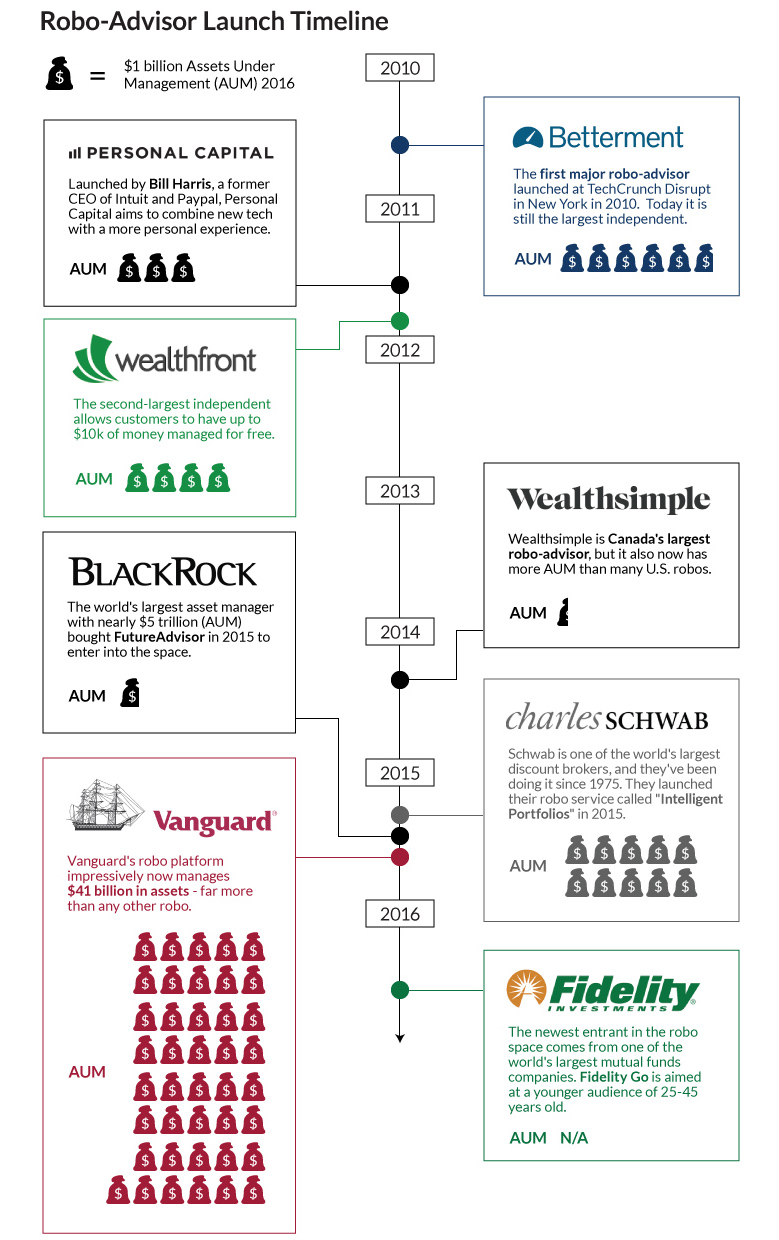
\includegraphics[height=0.9\textheight]{advisor}
        \caption{智能投顾发展一览 \newline (图片来源:http://www.visualcapitalist.com/robo-advisor-arms-race/)}
        \label{fig:adviosr}
\end{figure}



定义\\
发展\\
展望\\
visual 图片\\
选取国内外的资产\\
画出efficient frontier\\
给出配置组合\\



\chapter{实践出真知}

本节构建资产组合。
算法的理论基础是资本资产定价模型 CAPM (\textcolor{red}{TODO} 链接),
同时参考 wealthfront (\textcolor{red}{TODO} 链接) 的介绍。
算法主要通过 Python (\textcolor{red}{TODO} 链接)实现,
代码部分参考了通联数据(\textcolor{red}{TODO} 链接),
海外资产的数据由 Yahoo Finance (\textcolor{red}{TODO} 链接)提供,
国内资产的数据由 TuShare (\textcolor{red}{TODO} 链接)提供。

该算法的不足:(1)估算不同资产间的相关性;(2)预测资产的年化收益率。
事实上,上述两个问题是理论界与业界共同关心的主要问题。(\textcolor{red}{TODO} 链接)
本文主要用历史收益率来估算。

主要的资产组合都是ETF。
(\textcolor{red}{TODO} 解释为什么要用 etf)
手续费较低,流通性好,可以日内交易。
顺便提一下,\emph{华泰证券}~\footnote{此处不是广告!该券商未以任何形式提供赞助 -\_- }
 ETF 交易费最低 0.1 元!如果用来少量的搭建组合,还是比较划算。
其他券商还是最低 5 元。



\section{ETF 费用一览}

(\textcolor{red}{TODO} 各 etf 的管理费、规模、成立日期,管理人)

国内的 ETF 普遍比较坑,
QDII 组合费用(管理费+托管费)在 1.00\% 左右,
海外的约在 0.10\% 左右。


\section{Python Code}
代码:

\lstinputlisting[language=Python, caption = Download the data]{../02PythonCode/ETFDownloadData.py}

\lstinputlisting[language=Python, caption = Draw the captial allocation line]{../02PythonCode/ETFCAL.py}

\end{document}          

